\documentclass[12pt]{article}
\usepackage{lingmacros}
\usepackage{tree-dvips}
\usepackage{amsmath}
\usepackage{amssymb}
\usepackage{graphicx}
\usepackage{subcaption}

\begin{document}

\section*{Note sulla convergenza del metodo di newton con funzioni vettoriali}
Studiamo numericamente la convergenza di alcune funzioni vettorili. Questo studio verrà effetuato su una griglia $G$ di dimensione $56\times 6$ centrata in $[0,0]$ e di grana $k$.

\subsection{Calcoli preliminari}
Dato $v=[x,y]$ vettore di innsesco\\
Date le seguenti funzioni vettoriali:
\begin{gather}
	F_1(v) = 
	\begin{bmatrix}
		x^2-y^2-1\\
		x^2+y^2-2x-3
	\end{bmatrix}\label{F1}\\
	F_2(v)=
	\begin{bmatrix}
		\sin\left(\frac{\pi v_1}{2}\right)\\
		v_2
	\end{bmatrix}\label{F2}\\
	F_3(v) =
	\begin{bmatrix}
		2x_1+x_2-e^{-x_1}+1\\
		-x_1+2x_2-e^{-x_2}+1
	\end{bmatrix}\label{F3}
\end{gather}
Calcoliamone gli Jacobiani
\begin{gather*}
	J_1(v)=
	\begin{bmatrix}
		2x & -2y\\
		2x-2 & 2y
	\end{bmatrix}\\
	J_2(v)=
	\begin{bmatrix}
		\frac{\pi}{2}\cos\left(\frac{\pi v_1}{2}\right) & 0\\
		0 & 1
	\end{bmatrix}\\
	J_3(x)=
	\begin{bmatrix}
		2+e^{-x_1} & 1\\
		-1 & 2+e^{-x_2}
	\end{bmatrix}
\end{gather*}
Troviamo dove gli Jacobiani sono singolari:
\begin{itemize}
	\item $\det J_1(v) = 8y(x-1/2) = 0\iff x=1/2\ |\ y=0$
	\item $\det J_2(v) = \frac{\pi}{2}\cos\left(\frac{\pi x}{2}\right)=0 \iff x=2k+1,\ k\in\mathbb{Z}$
	\item $\det J_3(v) = (2+e^{-x})(2+e^{-y})+1 = 0$ non avviene mai
\end{itemize}
Troviamo analiticamente le soluzioni delle funzioni:
\begin{itemize}
    \item $F_1(v)=0 \iff (x,y)\in\{(-1,0),(2,\sqrt{3}),(2,-\sqrt{3})\}$
    \item $F_2(v)=0 \iff x=2k,\ y=0,\ k\in\mathbb{Z}$
    \item $F_3(v)=0 \iff (x,y)=(0,0)$
\end{itemize}

\subsection{Risultati}
Presenteremo ora i grafici di convergenza. Noto che in presenza di un pallino rosso il metodo non coverge.

\begin{figure}[htbp]
	\centering

	\begin{subfigure}{0.47\textwidth}
		\centering
		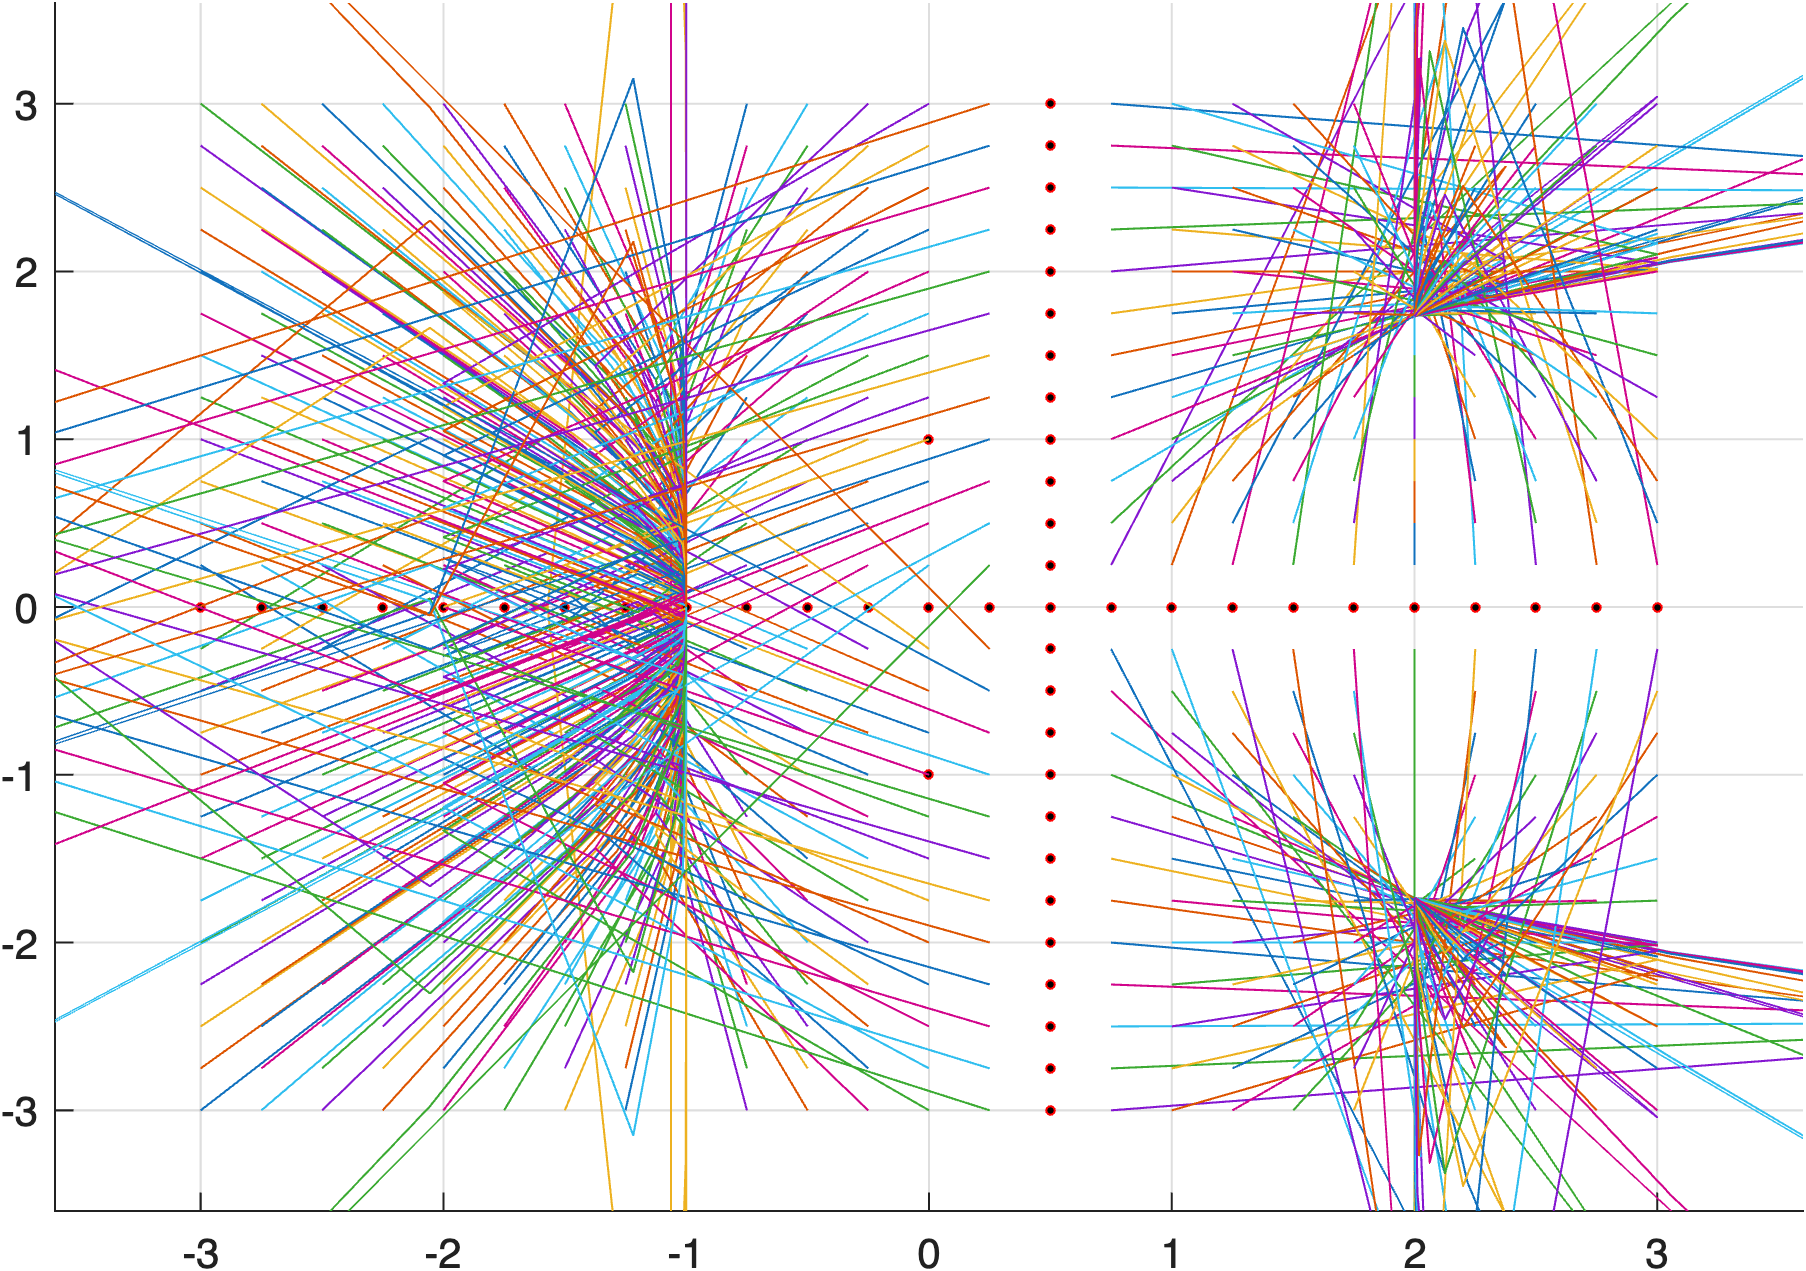
\includegraphics[width=\linewidth]{newton_plot.png}
		\caption{$F_1,\ k=25$}
	\end{subfigure}
	\hfill
	\begin{subfigure}{0.47\textwidth}
		\centering
		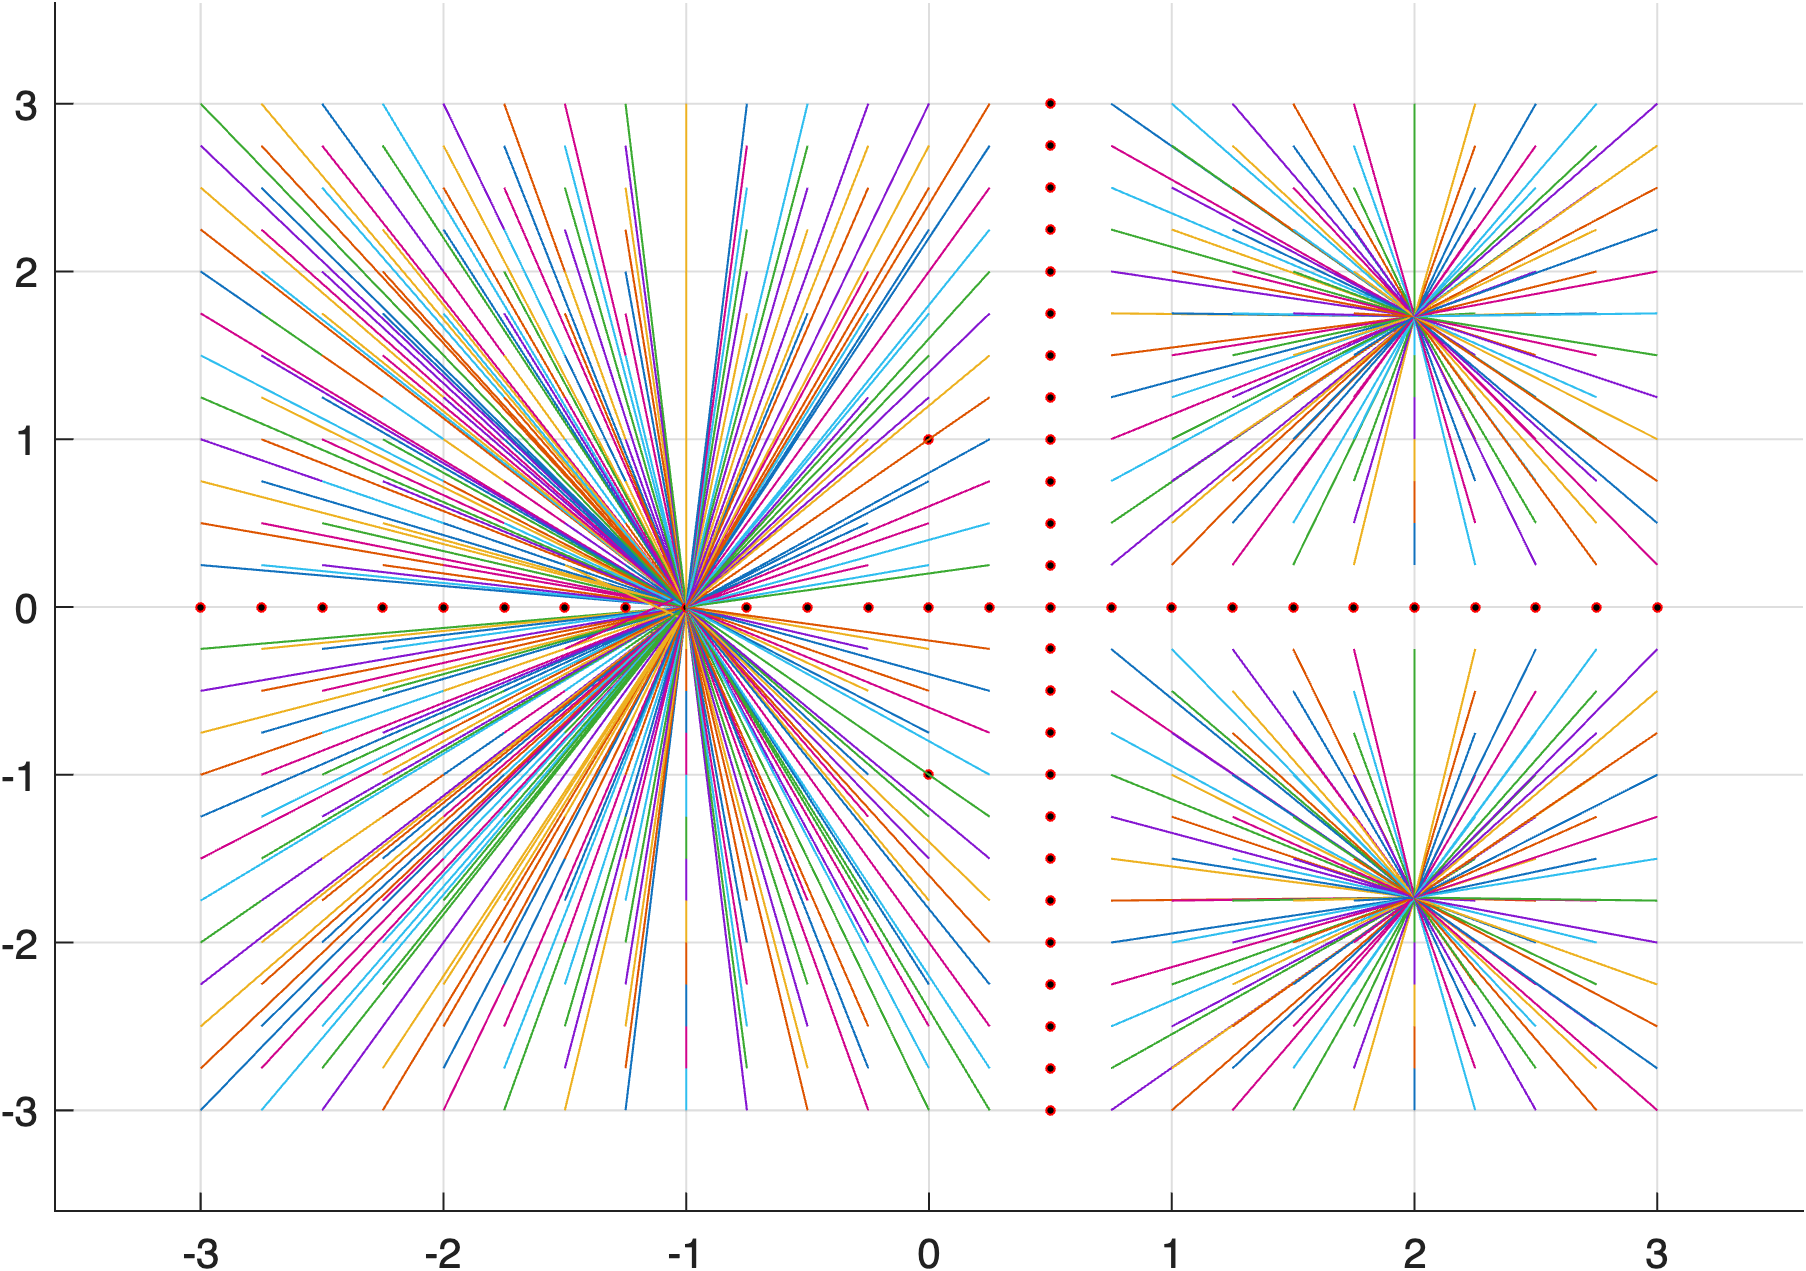
\includegraphics[width=\linewidth]{newton_plot_simp.png}
		\caption{$F_1,\ k=25$ (simp.)}
	\end{subfigure}

	\medskip

	\begin{subfigure}{0.47\textwidth}
		\centering
		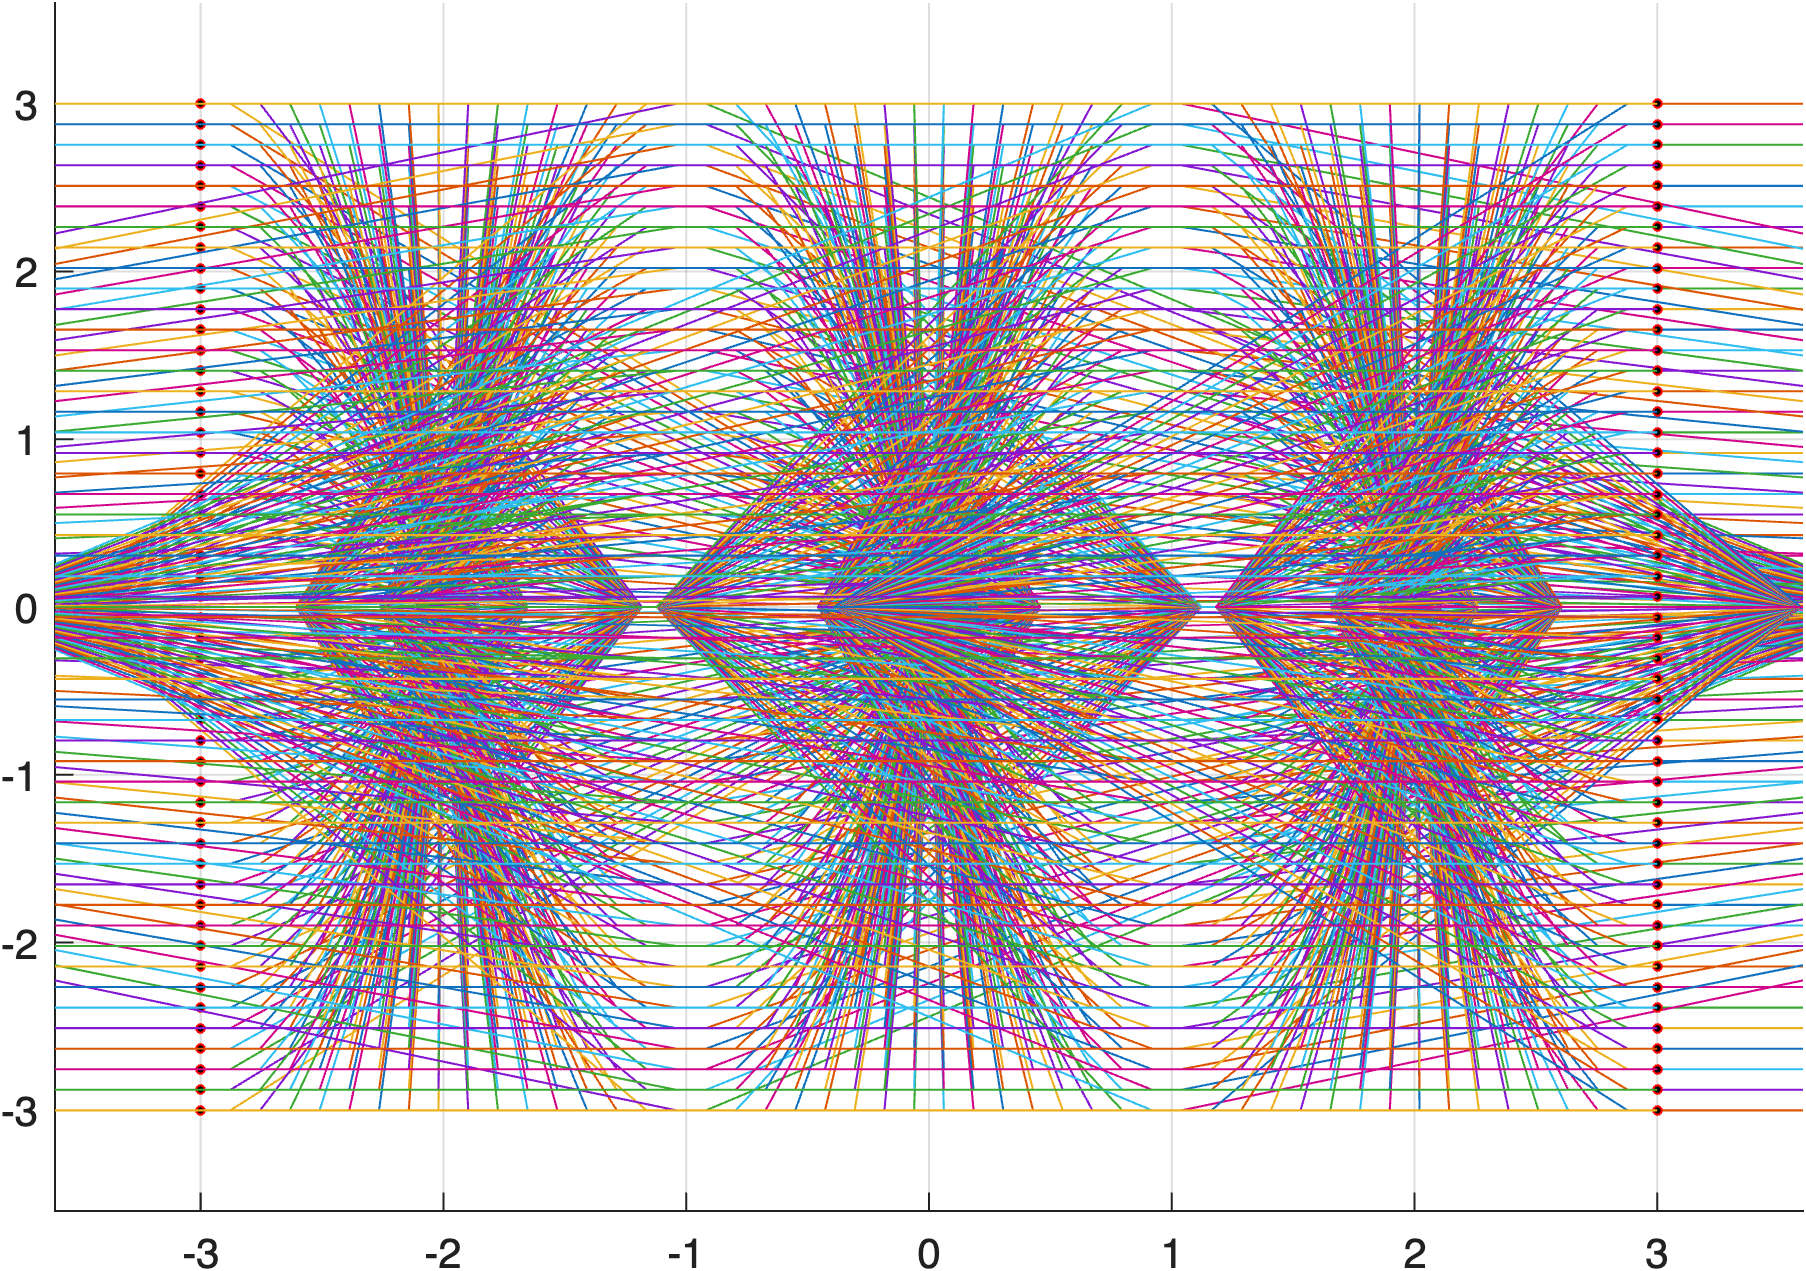
\includegraphics[width=\linewidth]{newton_plot1.png}
		\caption{$F_2,\ k=50$}
	\end{subfigure}
	\hfill
	\begin{subfigure}{0.47\textwidth}
		\centering
		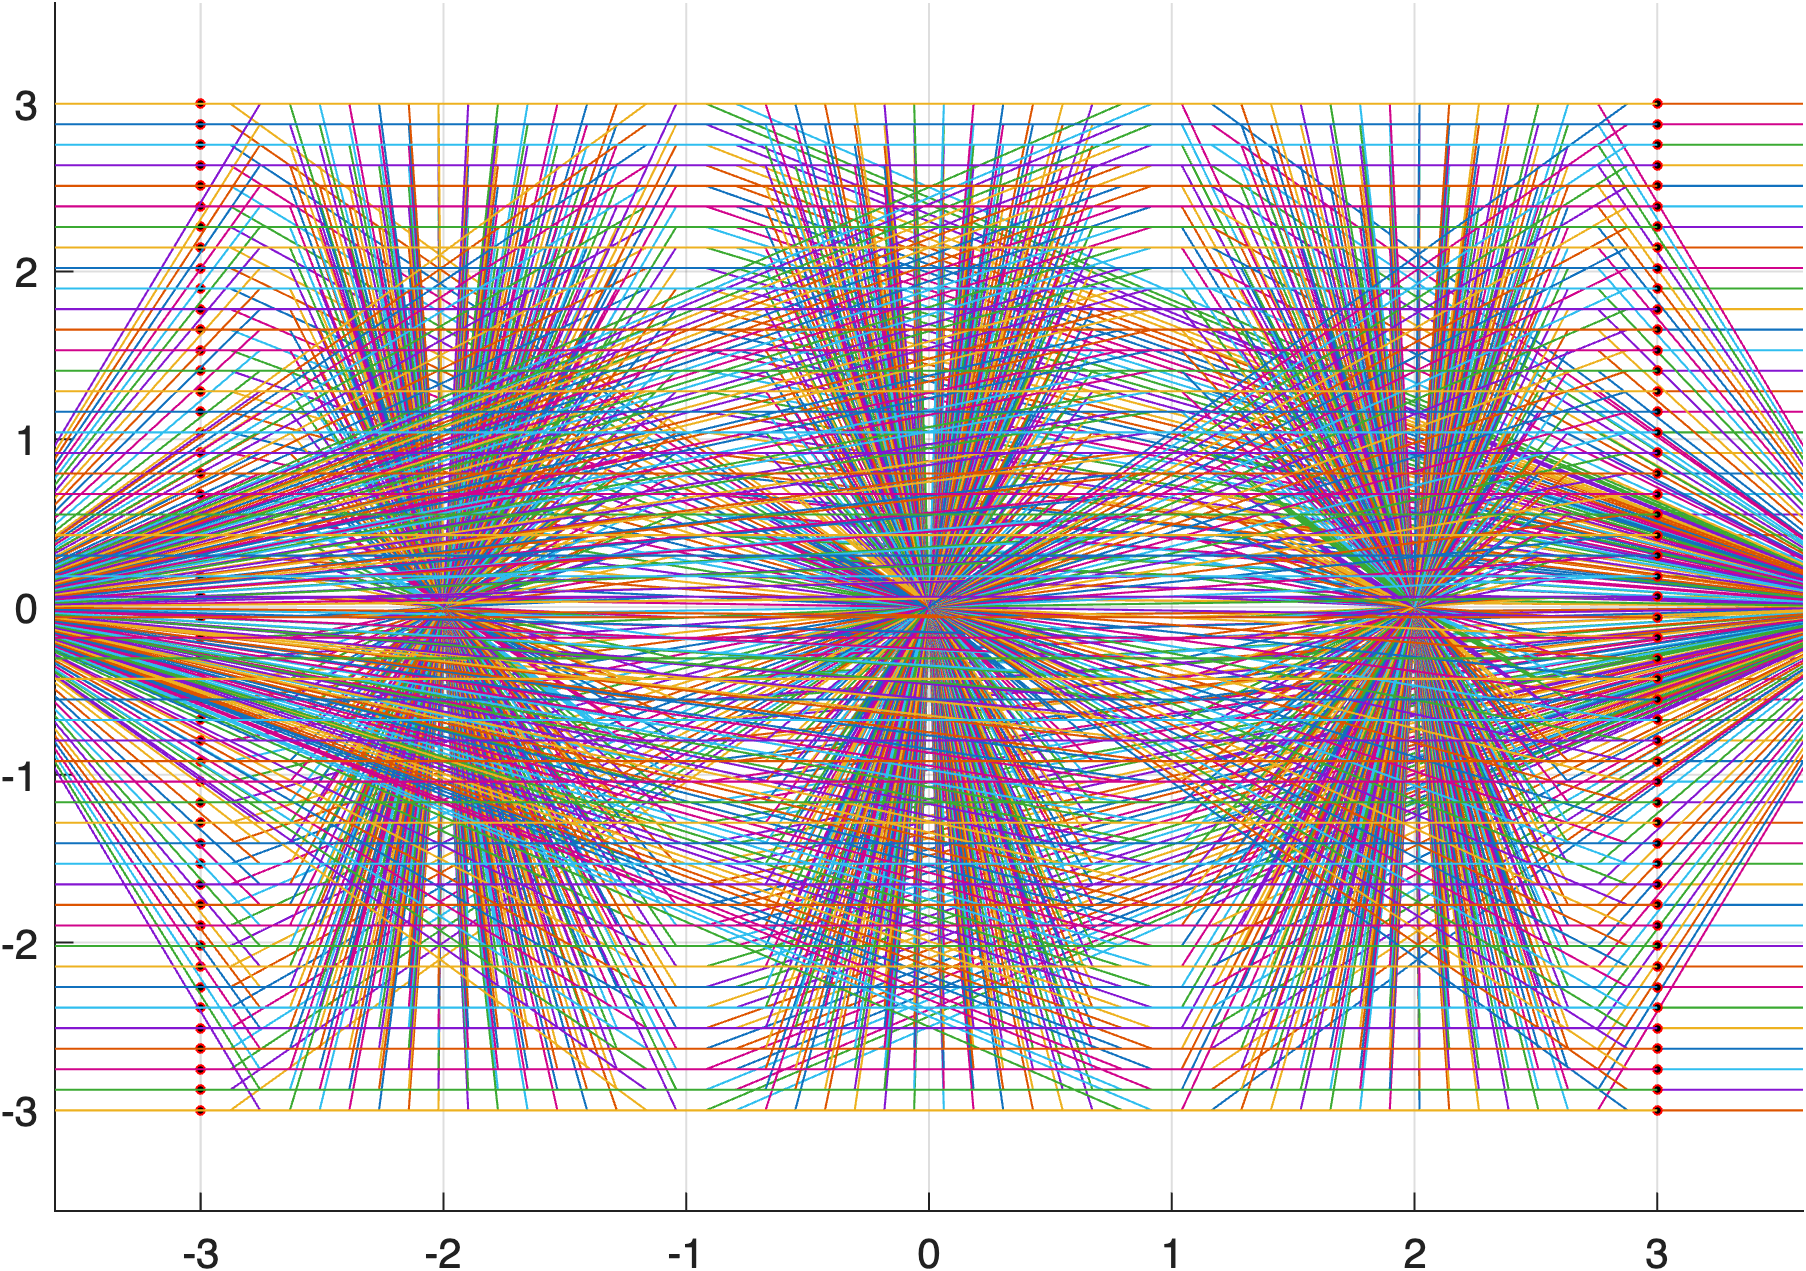
\includegraphics[width=\linewidth]{newton_plot_simp1.png}
		\caption{$F_2,\ k=50$ (simp.)}
	\end{subfigure}

	\medskip

	\begin{subfigure}{0.47\textwidth}
		\centering
		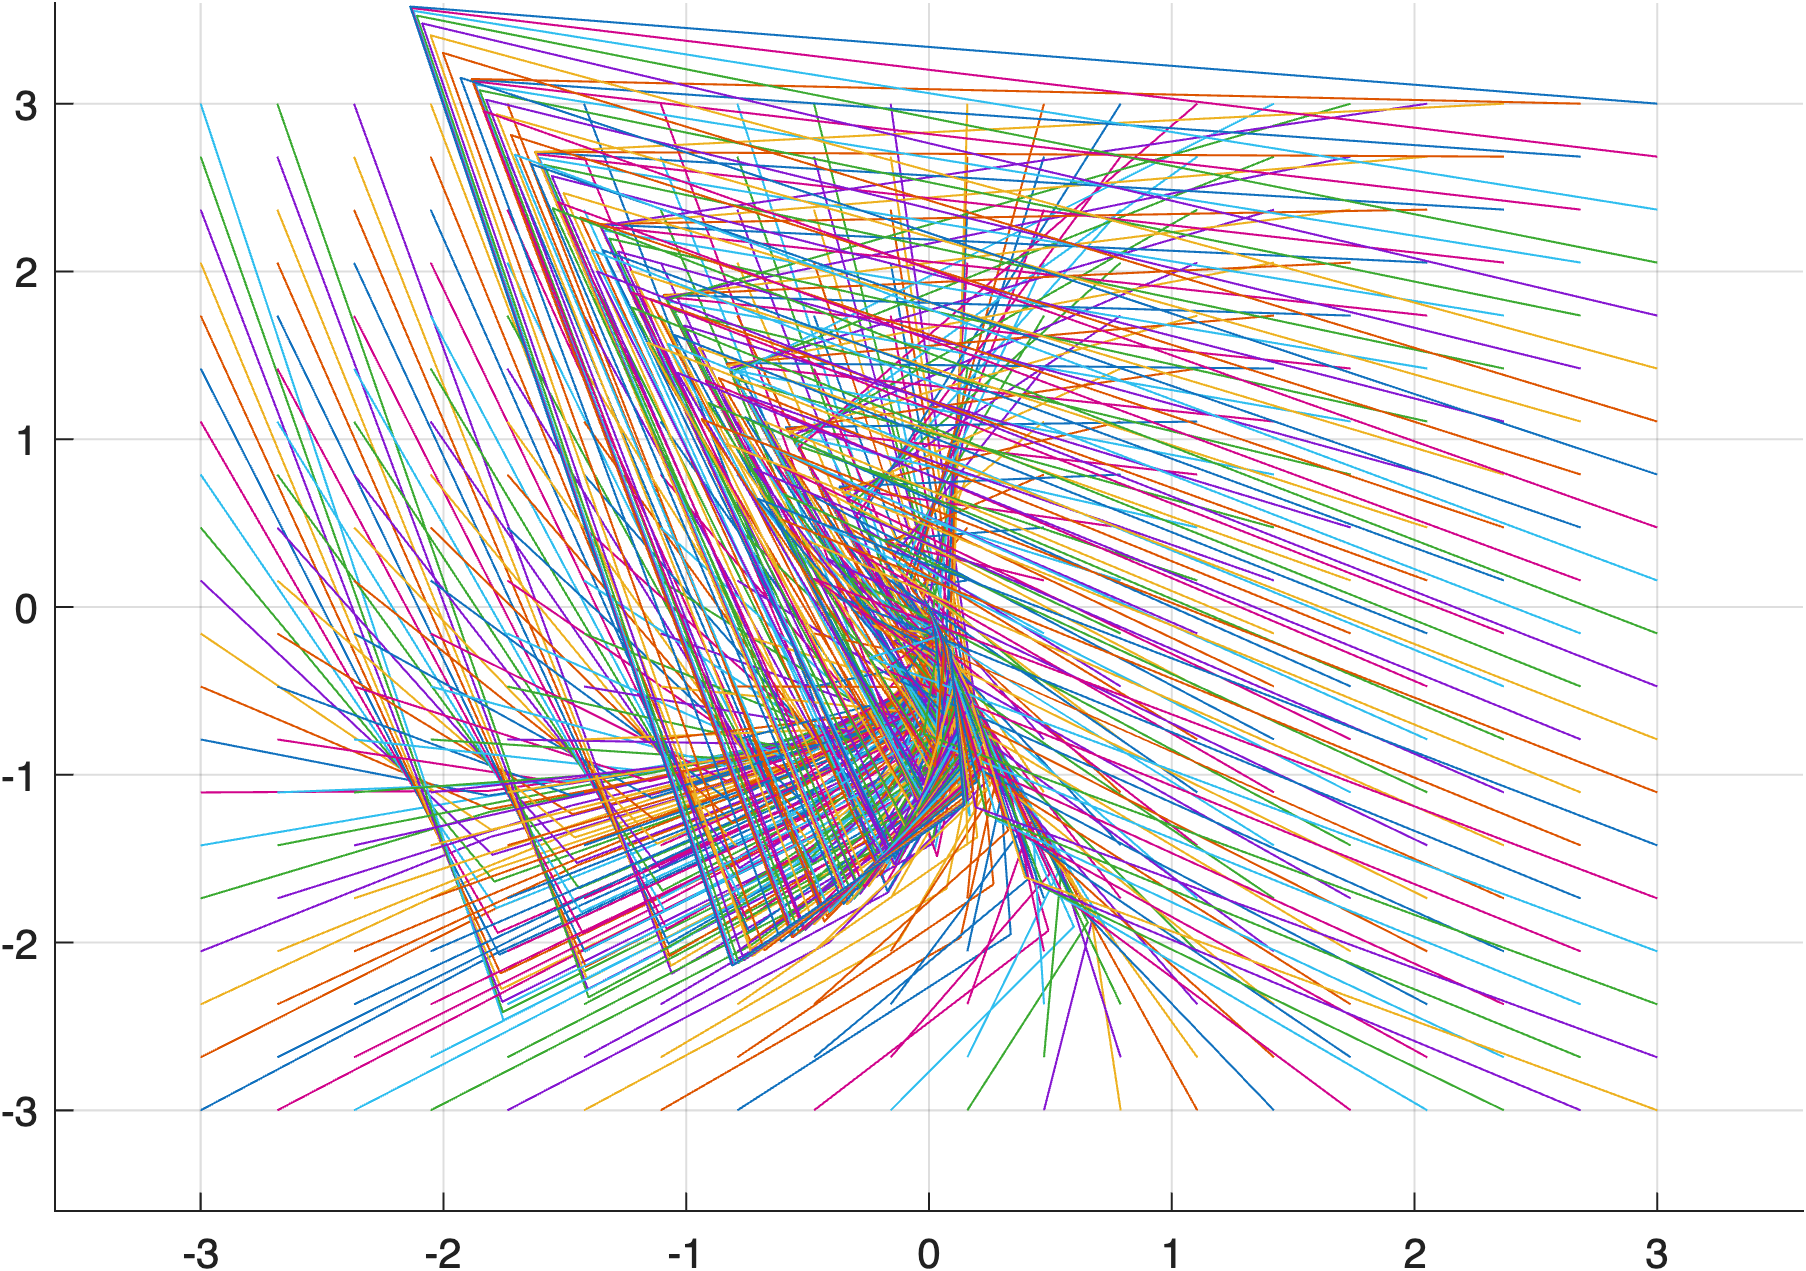
\includegraphics[width=\linewidth]{newton_plot2.png}
		\caption{$F_3,\ k=20$}
	\end{subfigure}
	\hfill
	\begin{subfigure}{0.47\textwidth}
		\centering
		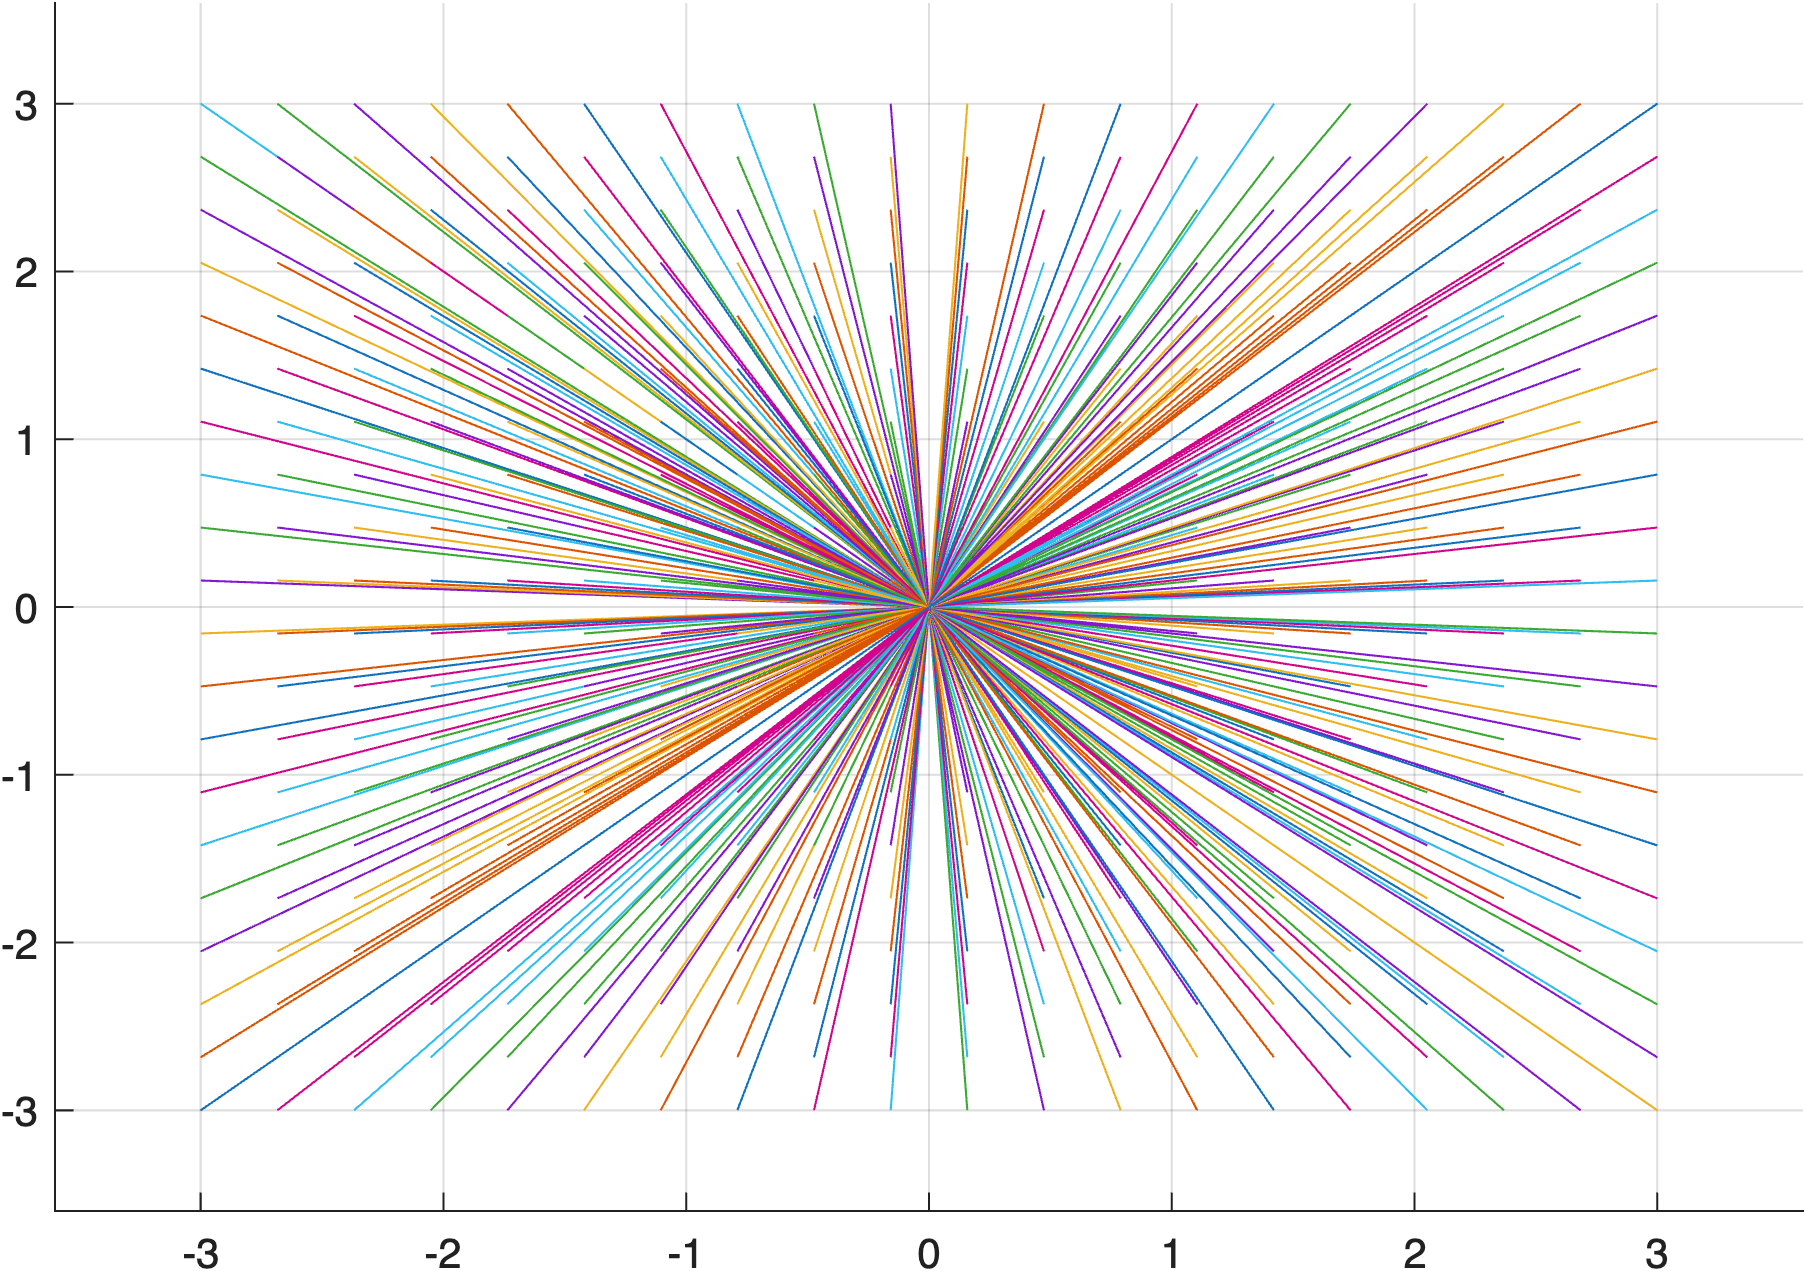
\includegraphics[width=\linewidth]{newton_plot_simp2.png}
		\caption{$F_3,\ k=20$ (simp.)}
	\end{subfigure}
	\caption{Grafici}
	\label{fig:newton}
\end{figure}

% \subsection{Considerazioni}
% Notiamo che lo spazio viene diviso in quattro settori delimitati dalle rette dove si anulla lo Jacobiano:
% \begin{enumerate}
% 	\item $x>1/2, y>0$ qui convergiamo a $[2,+\sqrt3]$
% 	\item $x>1/2, y<0$ qui convergiamo a $[2,-\sqrt3]$
% 	\item $x<1/2, y>0$ qui convergiamo a $[-1,0]$
% 	\item $x<1/2, y<0$ qui convergiamo a $[-1,0]$ 
% \end{enumerate}
% Possiamo dire che se stiamo in un settore con una radice abbiamo che la radice si comporta come un attattore per il metodo.
%
% Notiamo inoltre ce i punti $[0,1]$ e $[0,-1]$ sono segnalati come non convergenti infatti nella prima iterazione diventano $[-2,0]$ che come anticipato è un punto critico.

\end{document}


